%
% Presentación para congreso.
% Proyecto Lovelace.
%

\documentclass{beamer}
\usepackage{formato}
\newcommand{\Titulo}{Un vistazo a la tokenización}
%\renewcommand{\Subtitulo}{Primera Reunión de
%  Ciberseguridad para la Industria 4.0}
\newcommand{\Fecha}{Puebla, 14 de octubre de 2018}
\usepackage{formato_presentaciones}

\renewcommand{\Autor}{Daniel Ayala Zamorano \\\vspace{-2mm}
  {\tiny \texttt{daz23ayala@gmail.com}} \\
  Laura Natalia Borbolla Palacios \\\vspace{-2mm}
  {\tiny \texttt{ln.borbolla.42@gmail.com}} \\
  Ricardo Quezada Figueroa \\\vspace{-2mm}
  {\tiny \texttt{qf7.ricardo@gmail.com}} \\
  Sandra Díaz Santiago \\\vspace{-2mm}
  {\tiny \texttt{sdiazs@gmail.com}}}

\setbeameroption{show notes}

\begin{document}

  {\setbeamertemplate{footline}{}
  \frame{\titlepage}}

  \begin{frame}
    \frametitle{Contenido}
    \setcounter{tocdepth}{1}
    \tableofcontents
  \end{frame}

  % Espacio entre párrafos
  \setlength{\parskip}{0.5em}

  \section{El problema de la protección de datos bancarios}

  \begin{frame}{El problema de la protección de datos bancarios}
    \begin{itemize}
      \item El crecimiento del comercio en línea aunado a sistemas débilmente
        protegidos propició un incremento en los robos de datos bancarios.
      \item En el 2004 se publicó el PCI DSS\footnotemark.
      \item Hasta este momento el enfoque es proteger la información en todo
        lugar en el que se encuentre.
      \item A pesar de la publicación del estándar, las filtraciones de datos
        no han terminado.
    \end{itemize}
    \footnotetext{\textit{Payment Card Industry, Data Security Standard}}
  \end{frame}

  \section{¿Qué es la tokenización?}

  \begin{frame}{¿Qué es la tokenización?}
    \begin{itemize}
      \item Es la sustitución de datos sensibles por valores representativos
        sin una relación directa.
      \item Existen muchas empresas que proveen el servicio de tokenización,
        pero lo hacen sin detallar la forma en la que se realiza.
      \item En 2011 el PCI publicó las guías para la tokenización.
    \end{itemize}
  \end{frame}

  \section{Clasificación del PCI}

  \begin{frame}{Clasificación del PCI}
    \begin{figure}[H]
      \begin{center}
        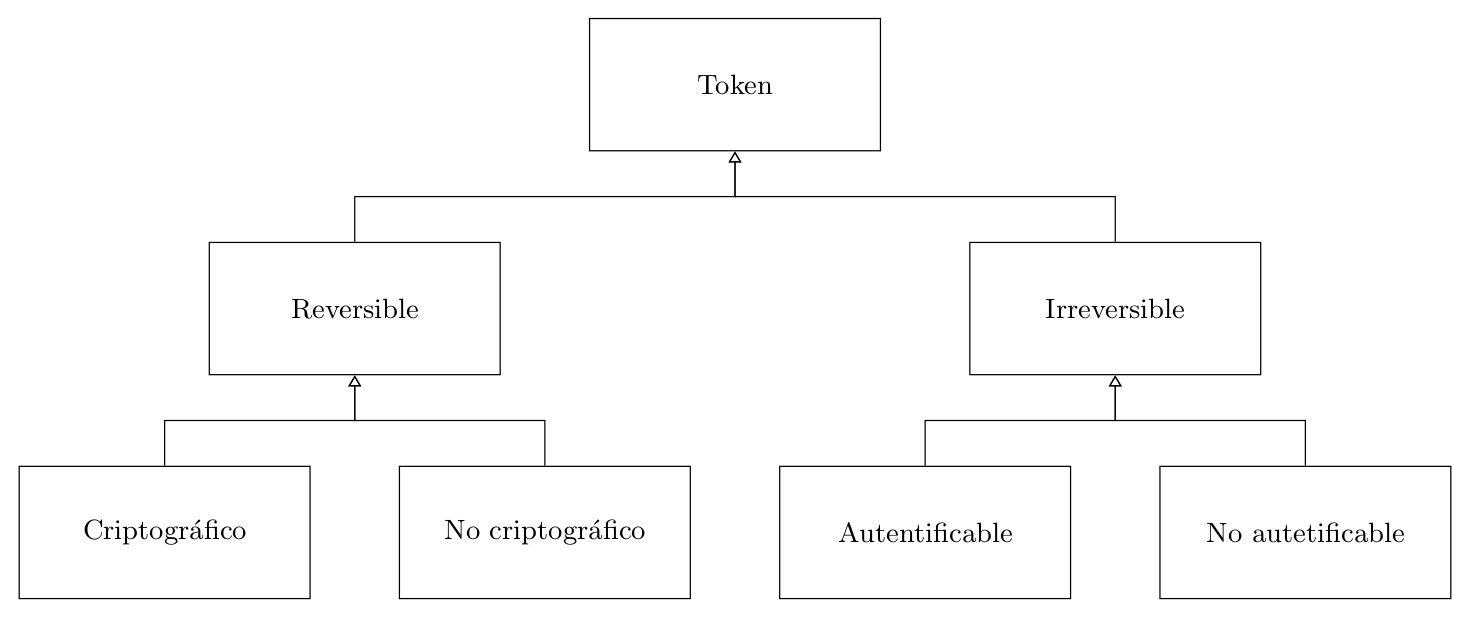
\includegraphics[width=0.8\linewidth]
          {presentacion_rci/diagramas/clasificacion_pci.png}
        \newline
        \newline
        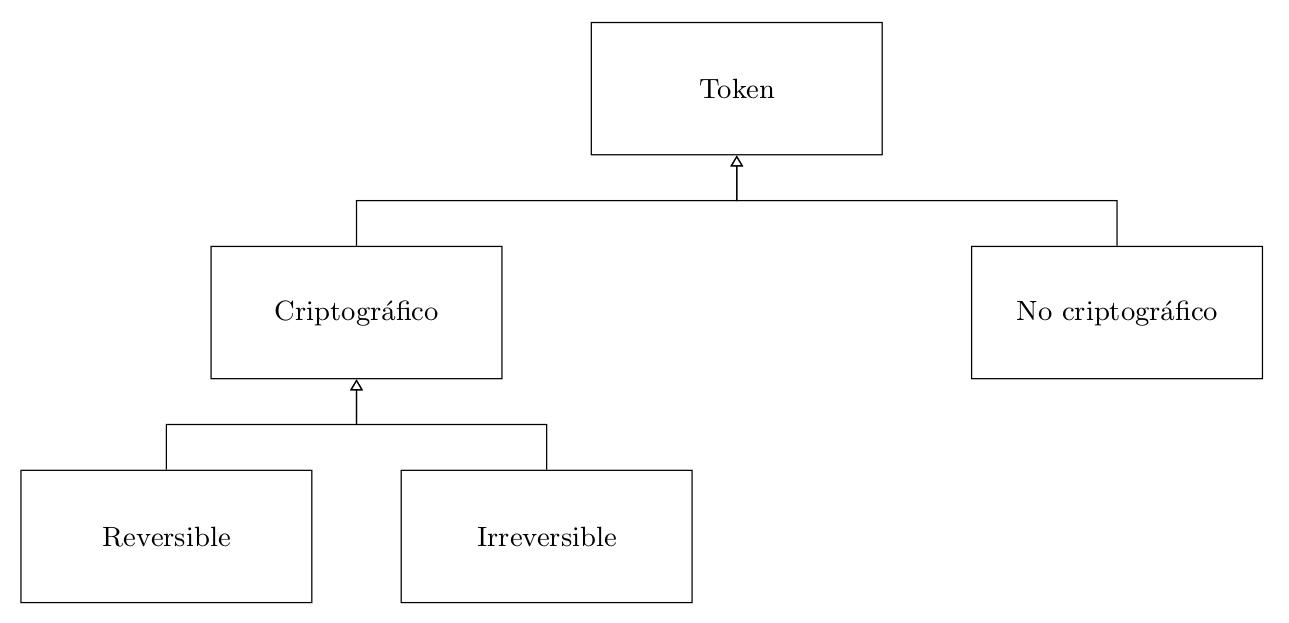
\includegraphics[width=0.8\linewidth]
          {presentacion_rci/diagramas/clasificacion_propia.png}
      \end{center}
    \end{figure}
  \end{frame}

  \section{Métodos reversibles: FFX y BPS}

  \begin{frame}{Métodos reversibles: FFX y BPS}

  \end{frame}

  \section{Métodos irreversibles: TKR, AHR y DRGB}

  \begin{frame}{Métodos irreversibles: TKR, AHR y DRGB}

  \end{frame}

  \section{Resultados y conclusiones}

  \begin{frame}{Resultados y conclusiones}

  \end{frame}

  \begin{frame}[allowframebreaks]{Bibliografía}
    \printbibliography
  \end{frame}

  % Espacio entre párrafos
  \setlength{\parskip}{0.0em}

  {\setbeamertemplate{footline}{}
  \frame{\titlepage}}

\end{document}
